\section{Methods}
\label{sec:study-one-methods}

\subsection{Study Design}

Describe the design in enough detail for a knowledgeable reader to reproduce the
study. Record the sampling strategy, inclusion and exclusion criteria, variables,
controls, preprocessing, model settings, software versions, random seeds, and
evaluation protocol where applicable. Explain why the design can answer the
research questions and identify any assumptions made before analysing the results.

The examples below demonstrate unified hyperlinks to \Cref{tab:datasets,fig:study-overview,fig:multi-panel,eq:example-score,alg:example}. Internal references, citations, and entries in the contents and lists use the same link treatment in the screen PDF.

\begin{definition}[Example score]
For observations $s_1,\ldots,s_N$, the aggregate score is the arithmetic mean defined in \Cref{eq:example-score}.
\end{definition}

\begin{equation}
  \operatorname{Score}=\frac{1}{N}\sum_{i=1}^{N}s_i,
  \label{eq:example-score}
\end{equation}

\begin{proposition}[Bounded aggregate]
If every observation satisfies $0\leq s_i\leq 1$, then the score in
\Cref{eq:example-score} also lies in $[0,1]$.
\end{proposition}

\begin{proof}
Summing the observation bounds gives $0\leq\sum_{i=1}^{N}s_i\leq N$.
Division by the positive integer $N$ proves the stated result.
\end{proof}

For a vector prediction $\bm{y}$ and target $\bm{t}$, a composite objective may be typeset as

\begin{align}
  \mathcal{L}(\bm{y},\bm{t})
    &= \lambda_1 \lVert \bm{y}-\bm{t} \rVert_1
     + \lambda_2 \bigl(1-\operatorname{sim}(\bm{y},\bm{t})\bigr), \\
  \lambda_1+\lambda_2 &= 1, \qquad \lambda_1,\lambda_2 \ge 0.
\end{align}

\subsection{Data and Procedure}

Summarise the origin and permitted use of each dataset, then document every split
or transformation that could affect the conclusions. Use a table for compact
dataset statistics and prose for decisions that require justification. A numbered
algorithm is useful when the procedure has branching, iteration, or an ordering
that must be reproduced.

\begin{table}[htbp]
  \centering
  \caption[Example dataset summary.]{Example dataset summary with aligned numeric columns. All names and values are placeholders and must be replaced.}
  \label{tab:datasets}
  \begin{threeparttable}
  \begin{tabular}{@{}l S[table-format=4.0] S[table-format=3.0] S[table-format=3.0]@{}}
    \toprule
    \textbf{Dataset} & {\textbf{Training}} & {\textbf{Validation}} & {\textbf{Test}} \\
    \midrule
    Example Alpha & 1000 & 200 & 300 \\
    Example Beta & 2400 & 400 & 600 \\
    Example Gamma\tnote{a} & 800 & 160 & 240 \\
    \bottomrule
  \end{tabular}
  \begin{tablenotes}[flushleft]\footnotesize
    \item[a] This note demonstrates explanatory material that belongs directly with a table.
  \end{tablenotes}
  \end{threeparttable}
\end{table}

\FloatBarrier

\begin{algorithm}[htbp]
  \caption{Example reproducible procedure}
  \label{alg:example}
  \begin{algorithmic}[1]
    \Require data $\mathcal{D}$, maximum iterations $T$, tolerance $\varepsilon$
    \Ensure fitted parameters $\bm{\theta}$
    \State initialise $\bm{\theta}$ and record the random seed
    \For{$t=1,\ldots,T$}
      \State compute the objective and update $\bm{\theta}$
      \If{the validation change is less than $\varepsilon$}
        \State \textbf{break}
      \EndIf
    \EndFor
    \State \Return $\bm{\theta}$
  \end{algorithmic}
\end{algorithm}
\FloatBarrier

\noindent\begin{minipage}{\linewidth}
\lstinputlisting[
  language=Python,
  caption={[Example analysis code.]Example analysis code loaded from a separate source file.},
  label={lst:example}
]{code/study-1/example-analysis.py}
\end{minipage}
\FloatBarrier

\subsection{Figures and Visual Evidence}

Figures should remain legible at their final printed size and should not depend on
colour alone. Supply descriptive captions, define symbols and abbreviations, and
refer to every figure from the surrounding discussion. The examples below exercise
a large full-width graphic and a multi-panel layout using standard
\verb|\includegraphics| commands. The example assets are stored under
\texttt{figures/study-1/}; authors can replace either the files or their paths.

\begin{figure}[htbp]
  \centering
  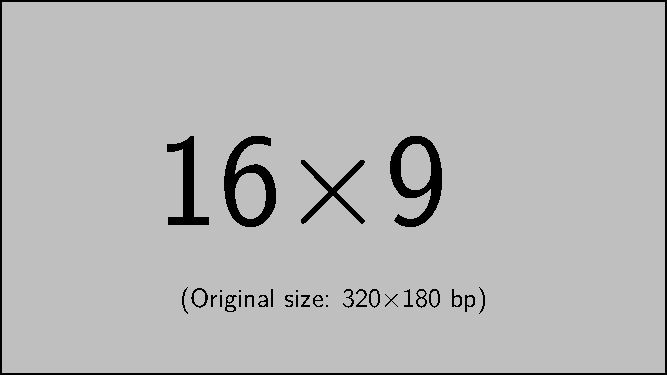
\includegraphics[width=0.88\textwidth]{figures/study-1/study-overview.pdf}
  \caption[Example full-width figure.]{Example full-width figure included from a PDF asset. Replace the file path with a legible, high-resolution PDF, PNG, or JPEG image.}
  \label{fig:study-overview}
\end{figure}

\begin{figure}[p]
  \centering
  \begin{subfigure}[t]{0.47\textwidth}
    \centering
    
\includegraphics[width=\linewidth]{figures/study-1/input.pdf}
    \caption{Input}
    \label{fig:panel-input}
  \end{subfigure}\hfill
  \begin{subfigure}[t]{0.47\textwidth}
    \centering
    
\includegraphics[width=\linewidth]{figures/study-1/reference.pdf}
    \caption{Reference}
    \label{fig:panel-reference}
  \end{subfigure}

  \vspace{5mm}

  \begin{subfigure}[t]{0.47\textwidth}
    \centering
    
\includegraphics[width=\linewidth]{figures/study-1/baseline.pdf}
    \caption{Baseline}
    \label{fig:panel-baseline}
  \end{subfigure}\hfill
  \begin{subfigure}[t]{0.47\textwidth}
    \centering
    
\includegraphics[width=\linewidth]{figures/study-1/proposed-result.pdf}
    \caption{Proposed result}
    \label{fig:panel-proposed}
  \end{subfigure}
  \caption[Example four-panel figure.]{Example four-panel figure. This caption deliberately tests \best{bold best-result text} and \runnerup{underlined runner-up text}; the plain optional caption keeps both styles out of the List of Figures.}
  \label{fig:multi-panel}
\end{figure}
\FloatBarrier
